\documentclass{ufsctex/ufsctex}

\usepackage{amsfonts, enumitem, tikz}

\newcommand{\hh}{$\mathcal{H}$}
\newcommand{\hash}[2][]{\mathcal{H}^{#1}(#2)}

\DeclareMathAlphabet{\mathcal}{OMS}{cmsy}{m}{n}

\def\precircle{(0.0, 0) circle (2.0cm)}
\def\seccircle{(2.5, 0) circle (2.0cm)}
\def\colcircle{(2.5, 0) circle (1.5cm)}

\colorlet{circle edge}{black!50}
\colorlet{circle area}{black!35}

\tikzset{
  filled/.style={fill=circle area, draw=circle edge, thick},
  outline/.style={draw=circle edge, thick}
}

\begin{document}

\instituicao[a]{Universidade Federal de Santa Catarina}
\departamento[o]{Departamento de Informática e Estatística}
\curso[o]{Programa de Graduação em Ciência da Computação}
\documento[a]{Monografia}
\titulo{
  Esquemas de assinatura digital baseados
  em funções de resumo criptográfico
}
\autor{Gustavo Zambonin}
\grau{Bacharel em Ciência da Computação}
\local{Florianópolis}
\data{27}{novembro}{2017}
\orientador[Orientador]{Prof. Dr. Ricardo Felipe Custódio}
\coorientador[Coorientador]{Prof. Dr. Daniel Panario}
\coordenador[Coordenador]{Prof. Dr. Rafael Luiz Cancian}

\numerodemembrosnabanca{1}
\orientadornabanca{nao}
\coorientadornabanca{nao}
\bancaMembroA{
  Lucas Pandolfo Perin, M.Sc. \\
  Universidade Federal de Santa Catarina
}

\dedicatoria{Às mulheres da minha vida}

\agradecimento{...}

\epigrafe{
  \emph{Look at you, hacker: a pathetic creature of meat and bone,
  panting and sweating as you run through my corridors.
  How can you challenge a perfect, immortal machine?}
}{SHODAN (System Shock 2, 1999)}

\textoResumo{
  Algoritmos utilizados em esquemas de assinatura digital atualmente, como RSA
  e ECDSA, têm sua segurança baseada na dificuldade de calcular a fatoração
  de números muito grandes ou logaritmos discretos. Este tipo de cômputo pode
  ser realizado por um computador quântico suficientemente poderoso, utilizando
  algoritmos já conhecidos (e.g. algoritmo de Shor). Deste modo, para manter
  o ambiente de assinaturas digitais continuamente seguro, é necessário oferecer
  alternativas pós-quânticas, ou seja, resistentes a computadores quânticos.
  Este trabalho busca apresentar esquemas baseados apenas em funções de resumo
  criptográfico, cuja segurança baseia-se apenas na resistência à colisão da
  função escolhida, com o objetivo de mostrar que a construção de esquemas de
  assinatura seguros independe de problemas considerados difíceis em teoria de
  números ou álgebra, levando em conta apenas algoritmos quânticos, como o
  algoritmo de Grover. Ademais, discutem-se soluções para alguns problemas
  deste tipo de esquema, como o tamanho e possibilidade de reutilização das
  chaves pública e privada, assim como uma variada gama de algoritmos com estas
  características, na forma de novos esquemas, particularmente os baseados em
  árvores de Merkle e esquema Winternitz.
}
\palavrasChave{
  criptografia pós-quântica, Merkle, assinatura digital, Winternitz,
  resumo criptográfico, funções de resumo
}

\textAbstract{
  Algorithms currently used in digital signature schemes, such as RSA and
  ECDSA, base their security on the difficulty of calculating large integer
  factorizations or discrete logarithms. This kind of computation can be
  achieved through a sufficiently powerful quantum computer running already
  known algorithms, such as Shor's. Hence, to keep digital signatures secure,
  it is imperative to offer post-quantum alternatives, that is, resistant to
  quantum computers.  This work explores hash-based digital signature schemes,
  whose security is reduced to the collision resistance of a chosen hash
  function, with the aim of showing that the construction of such secure
  schemes is independent from hard problems from number theory or algebra,
  considering only quantum algorithms, e.g. Grover's. Furthermore, some
  problems for these schemes are introduced and discussed (some of which are
  the size and repeated usage of the public and private keys), and also various
  algorithms in the shape of new schemes, notably the ones based on Merkle
  trees and variants of Winternitz.
}
\keywords{
  post-quantum cryptography, Merkle, digital signature, Winternitz,
  digest, hash functions
}

\chapter{Introdução}

A aplicação de protocolos criptográficos é essencial no contexto da validação e
proteção de quaisquer comunicações realizadas por um conjunto de entidades,
sejam estas dispositivos eletrônicos ou indivíduos, em virtude da possível
criticalidade e sensibilidade atribuídas aos dados transmitidos. Esquemas de
assinatura digital são comumente utilizados para assegurar este processo de
maneira formal \cite{Goldreich:2004:FCV:975541}, através da autenticidade e
não-repúdio do remetente e certeza da integridade dos dados em, a fim de
traduzir o resguardo provido por uma assinatura de próprio punho no mundo real.

Na prática, a maior parte destes esquemas utilizam como alicerce algorítmico
criptossistemas assimétricos baseados em problemas `'difíceis`' da teoria
dos números, como a fatoração de inteiros ou resolução do logaritmo discreto,
ambos para números grandes. Este fato provê a segurança necessária para os
esquemas em computadores clássicos (eletrônicos), por conta da inexistência de
algoritmos que resolvem estes problemas em tempo polinomial, até o momento.
Entretanto, em computadores quânticos, algoritmos dessa forma já existem - em
especial, o algoritmo de Shor \cite{Shor:1997:PAP:264393.264406} - efetivamente
tornando estes esquemas clássicos inseguros neste novo contexto.

Para combater esta situação, a criptografia pós-quântica encarrega-se de buscar
algoritmos criptográficos cuja segurança é considerada suficiente mesmo
utilizando-se de um computador quântico e ataques especializados, como o
algoritmo de Grover \cite{Grover:1996:FQM:237814.237866}. Esta área conta com
diversas abordagens diferentes: a criptografia baseada em reticulados,
polinômios multivariados sobre um corpo finito, códigos de correção de erros,
morfismos entre curvas elípticas supersingulares e criptossistemas simétricos.
Entretanto, reduções de segurança formais não existem para alguns destes
métodos, e para outros, o tamanho das chaves impossibilita a utilização destes
em aplicações práticas.

Não obstante, uma abordagem distinta de esquema de assinatura digital
resistente a computadores quânticos pode ser obtida apenas com funções de
resumo criptográfico, construídas a partir de funções de mão única
\cite{cryptoeprint:2005:328}. De fato, estas funções, desde que apresentem
requisitos de segurança como resistência à segunda pré-imagem e à colisões, são
necessárias e suficientes para a construção de esquemas bem comportados e
seguros \cite{Rompel:1990:OFN:100216.100269}. Visto que estas funções são
estudadas exaustivamente por conta de sua vasta presença em diversos âmbitos da
segurança da informação, reduções de segurança são mais comuns em relação a
outras abordagens pós-quânticas, e tamanhos de chaves e assinaturas não são
proibitivos.

Esquemas de assinatura digital baseados em funções de resumo criptográfico
consistem da utilização de um esquema de assinatura digital única, onde apenas
uma mensagem pode ser assinada de modo seguro, ou sua combinação com a
estrutura de dados chamada de árvore de Merkle
\cite{Merkle:1989:CDS:118209.118230}, que abriga diversos pares de chave do
esquema supracitado como suas folhas, e reduz a verificação destes para uma
única chave, codificada em sua raiz. Esta árvore é construída com a
concatenação de resumos criptográficos do conteúdo dos nós, habilitando assim a
assinatura de diversas mensagens. Como uma função específica não é necessária,
é possível obter uma grande variedade de esquemas, garantindo a versatilidade
destas abordagens.

Embora os esquemas iniciais tenham sido construídos sem atenção particular à
eficiência de modo geral (e.g. o esquema de assinatura única de Lamport-Diffie
\cite{Lamport1979} assina apenas um \emph{bit} de informação em sua forma mais
simples), muitos resultados práticos demonstram a redução contínua do tempo de
verificação da assinatura, tamanho e tempo para geração do par de chaves e
assinatura, bem como avanços teóricos possibilitam a utilização de funções com
requisitos de segurança mínimos, garantem o conceito de sigilo encaminhado
\cite{Buchmann:2011:XPF:2184003.2184011} (i.e. comprometimento de uma chave não
implica na segurança de mensagens que utilizaram esta chave anteriormente) e da
ausência de estado \cite{Bernstein2015} (i.e. esquema não necessita registrar
quais chaves de assinatura única já foram utilizadas).

Neste trabalho, será estudada bibliografia referente aos temas abordados,
buscando encontrar as vantagens e desvantagens de cada um dos esquemas
de assinatura digital escolhidos, bem como observar seu desempenho e tamanho
de elementos como par de chaves e assinatura, ao utilizar funções de resumo
criptográfico distintas em implementações produzidas ou fornecidas.
Elaborar-se-á uma comparação exaustiva dos esquemas de assinatura única e
baseados em árvores de Merkle a fim de demonstrar a evolução recorrente
destes algoritmos.

\section{Objetivos}

\begin{itemize}

  \item \emph{Objetivo geral.} Apresentar um estudo detalhado sobre esquemas
    de assinatura digital baseados em funções de resumo criptográfico,
    partindo de esquemas de assinatura única \cite{Lamport1979}, observando
    o refinamento destes, até o estado da arte, onde não é necessário saber
    quantas assinaturas foram geradas anteriormente \cite{Bernstein2015}, bem
    como implementações em linguagem de alto nível para a fácil compreensão
    destes esquemas.

  \item \emph{Objetivos específicos.} Descrever os esquemas de assinatura
    digital única Lamport-Diffie e Winternitz, e variantes; descrever os
    esquemas de assinatura digital baseado em árvores de Merkle: \emph{Merkle
    Signature Scheme}, \emph{eXtended Merkle Signature Scheme}, SPHINCS;
    implementar os esquemas supracitados; comparar o desempenho destes,
    utilizando funções de resumo criptográfico e parâmetros internos aos
    algoritmos distintos, onde aplicável.

\end{itemize}

\chapter{Primitivas criptográficas}

\section{Funções de resumo criptográfico}

Uma função de resumo \hh{} mapeia valores deterministicamente entre dois
conjuntos. O domínio pode ter tamanho infinito, e neste caso a função pode ser
chamada de função de compressão; a imagem deve ser estritamente menor do que o
domínio e finita, e elementos deste conjunto são chamados de resumos. É
desejável para \hh{} que estes mapeamentos ocorram de tal maneira que não
ocorra uma relação aparente entre entradas e saídas da função. Funções de
resumo adicionadas de propriedades que tornam-as adequadas para utilização no
contexto de segurança da informação são chamadas de funções de resumo
criptográfico, e possibilitam a certeza da integridade de dados, mesmo que
armazenados em um dispositivo inseguro.

Tome $X : \{0, 1\}^{*}$ e $Y : \{0, 1\}^{n}$, $n \in \mathbb{N}$. Então,
$\mathcal{H} : X \longrightarrow Y$. De acordo com
\cite{stinson2005cryptography}, para que qualquer \hh{} seja considerada
criptográfica, deve ser difícil resolver os três problemas listados abaixo.
É importante notar que um problema é considerado `'difícil`', ou
computacionalmente impraticável, quando o tempo ou recursos gastos para esta
computação excedem a validade ou utilidade da informação desejada.

\begin{enumerate}[label=\roman*.]

  \item Fornecido um resumo $h \in Y$, achar a mensagem original $m \in X$ que
    gerou $h$ através de $\hash{m} = h$; \hh{} é considerada resistente à
    pré-imagem (\textsc{Pre}) se isto não pode ser resolvido de maneira
    eficiente.

  \item Fornecida uma mensagem $m_0 \in X$, achar uma mensagem $m_1 \in X$ tal
    que $m_0 \neq m_1$ e $\hash{m_0} = \hash{m_1}$. \hh{} é considerada
    resistente à segunda pré-imagem (\textsc{Sec}) se isto não pode ser
    resolvido de maneira eficiente.

  \item Para quaisquer duas mensagens $m_0, \; m_1 \in X$ e $m_0 \neq m_1$,
    $\hash{m_0} = \hash{m_1}$. \hh{} é considerada resistente à colisões
    (\textsc{Col}) se isto não pode ser resolvido de maneira eficiente.

\end{enumerate}

Note que ii. e iii. apresentam uma sutil diferença: no primeiro, um adversário
não pode escolher $m_0$, enquanto no segundo, quaisquer pares de mensagens
podem ser testados. A resistência à colisão, portanto, implica na resistência
à segunda pré-imagem, visto que basta um adversário fixar $m_0$ para simular
o cômputo de $m_1$. Outra característica desejada é o efeito avalanche,
baseado no conceito de difusão (\cite{Stallings:2010:CNS:1824151}): trocar
apenas um \emph{bit} da mensagem $m$ deve modificar cerca de metade dos
\emph{bits} do resumo, e vice-versa.

\begin{figure}[htbp]
  \centering
  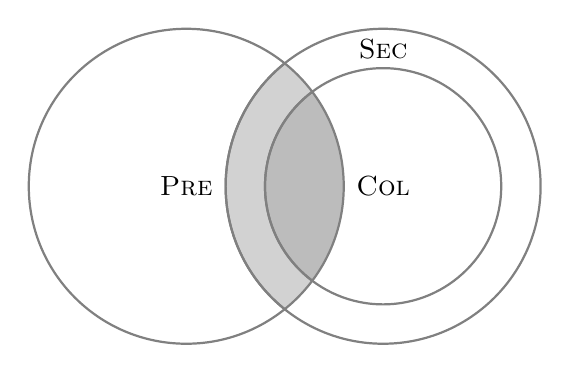
\begin{tikzpicture}
    \begin{scope}[fill opacity=0.5]
      \clip \precircle;
      \fill[filled] \seccircle;
      \fill[filled] \colcircle;
    \end{scope}
    \draw[outline] \precircle node {\textsc{Pre}};
    \draw[outline] \seccircle node {};
    \draw node[right=2.5cm, above=1.5cm] {\textsc{Sec}};
    \draw[outline] \colcircle node {\textsc{Col}};
  \end{tikzpicture}
    \caption{Diagrama de Venn das resistências de uma função de resumo
      criptográfico.}
    \label{fig:1}
\end{figure}

% falar de ataques (colisao, preimagem)
% explicitar pq tem uma area cinza e relacionar com os esquemas
% escrever a introducao desse capitulo

\subsection{Construção Merkle--Damgård}

\subsection{Construção esponja}

\section{Criptografia simétrica}

\section{Criptografia assimétrica}

\subsection{RSA}

\section{Assinatura digital}

\bibliographystyle{abnt-alf}
\bibliography{ref}

\end{document}
